\documentclass[12pt,a4paper]{report}
\usepackage{tikz}
\usetikzlibrary{calc,arrows.meta,positioning}

\tikzset{
    every node/.style={font=\sffamily\small},
    main node/.style={thick,circle,draw,font=\sffamily\Large}
}

\begin{document}
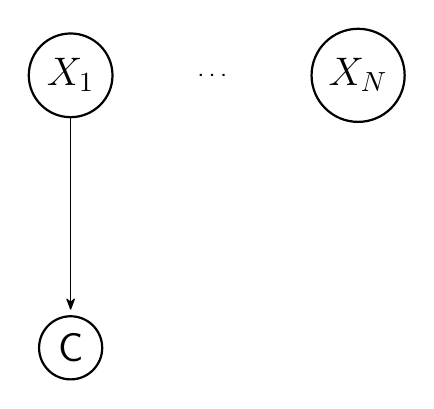
\begin{tikzpicture}[->,>={Stealth[round,sep]},shorten >=1pt,auto,node distance=2.5cm]

    \node[main node] (1) {$X_1$};
    \node[main node] (2) [right =of 1]{$X_N$};
    \node[main node] (5) [below =of 1]{C};

    \node at ($(1)!.5!(2)$) {\ldots};

    \draw (1) -- (5);
\end{tikzpicture}
\end{document}